\section{Zielsetzung}
\label{sec:Zielsetzung}

Ziel des Versuches ist die Bestimmung der Diffusionskonstante von Wasser.
Diese wird mittels gepulster \emph{Kernspinresonanz} (NMR) ermittelt,
indem also der zeitliche Verlauf einer Magnetisierung der Probe unter
Einstrahlung eines Hochfrequenzfeldes untersucht wird.
Dabei treten Relaxationsprozesse auf, die unter Verwendung zweier
Relaxationszeiten charakterisiert werden.

\section{Theorie}
\label{sec:Theorie}

\subsection{Magnetisierung einer Probe}
\label{sec:TheoMagnetisierung}

Im Folgenden wird die Magnetisierung einer Probe erläutert, die im thermischen
Gleichgewicht mit ihrer Umgebung steht.
Anschließend wird auf die Larmor-Präzession näher eingegangen.

Beim Anlegen eines externen Magnetfelds $\vec{B}_0 = B_0 \vec{e}_\text{B}$ eines ansonsten
feldfreien Raums spalten die Kernspinzustände der Probe in $2S+1$ Unterniveaus auf.
Dabei zeige das Magnetfeld in $z$-Richtung und $S$ bezeichne die Spinquantenzahl der
Zustände, die mittels der Orientierungsquantenzahl $m$ unterschieden werden.
Im thermischen Gleichgewicht sind die Zustände nach der Maxwell-Boltzmann-Verteilung
und damit ungleichmäßig besetzt.
Aufgrund der Orientierung der einzelnen Spins ergibt sich daraus eine Kernspinpolarisation
$\left<S_\text{z}\right>$.
Bei der Betrachtung von Protonen mit $S = \sfrac{1}{2}$ und der Abschätzung
$m \gamma B_0 \ll k_\text{B} T$ ergibt sich in linearer Näherung
\begin{equation*}
  \left<I_\text{z}\right> = -\frac{\hbar^2}{4}\frac{\gamma B_0}{k_\text{B} T}.
\end{equation*}
Dabei bezeichnet $\gamma$ das gyromagnetische Verhältnis des Kerns,
$k_\text{B}$ die Boltzmann-Konstante, $T$ die Temperatur
und $\hbar$ das reduzierte Plancksche Wirkungsquantum.
% TODO: Überlegen, ob hier ein Satz zu m=+-0.5 mit Energieaufspaltung eingefügt werden könnte
Aufgrund der Verknüpfung der Kernspinpolarisationen der Kerne
mit dem magnetischen Moment $\vec{\mu_\text{S}}$ folgt aus der ungleichmäßigen
Besetzung eine makroskopische Magnetisierung $\vec{M_0}$,
deren Erwartungswert in Richtung des äußeren Feldes
\begin{equation*}
  M_0 = \frac{1}{4} \mu_0 \gamma^2 \frac{\hbar^2}{k_\text{B}} N \frac{B_0}{T}
\end{equation*}
beträgt.
Dabei bezeichnet $\mu_0$ die Permeabilität des Vakuums und
$N$ die Anzahl der Momente pro Volumeneinheit.

% Larmor-Präzession
Für die NMR-Spektroskopie ist interessant, wie sich die Magnetisierung $\vec{M}$
der Probe nach einer Auslenkung aus der Gleichgewichtslage $\vec{M_0}$
zeitlich entwickelt.
Aufgrund der großen Anzahl von Einzelmomenten
($N$ in Größenordnung \SI[retain-unity-mantissa=false]{1e28}{\per\cubic\meter})
lässt sich diese Entwicklung klassisch behandeln.
Auf die Magnetisierung der Probe wirkt im externen Magnetfeld ein Drehmoment
$\sim \vec{M} \times \vec{B}$,
welches zu einer Präzessionsbewegung der Magnetisierung um die Achse des
Magnetfelds führt.
Diese Präzession wird Larmor-Präzession und die zugehörige Kreisfrequenz
\begin{equation}
  \omega_\text{L} = \gamma B_0
  \label{eqn:LarmorFrequenz}
\end{equation}
wird Larmor-Frequenz genannt.

% Relaxation
Neben der Präzession um das externe Magnetfeld treten Relaxationseffekte auf.
Wird die Magnetisierung aus der Gleichgewichtslage $\vec{M}_0$ entfernt,
strebt sie nach dem Verschwinden der auslösenden Störung wieder zu dieser zurück.
Diese Relaxationseffekte können durch zwei Zeitkonstanten $T_1$ und
$T_2$ charakterisiert werden.
% Beschrieben wird dieser Vorgang mit den Differentialgleichungen
% \begin{align*}
  % \frac{\symup{d} M_\text{z}}{\symup{d} t} &= \frac{M_0 - M_\text{z}}{T_1} \\
  % \frac{\symup{d} M_\text{x}}{\symup{d} t} &= -\frac{M_\text{x}}{T_2} \\
  % \frac{\symup{d} M_\text{y}}{\symup{d} t} &= -\frac{M_\text{y}}{T_2}.
% \end{align*}
Dabei bezeichnet die Zeitkonstante $T_1$ die sogenannte longitudinale oder
Spin-Gitter-Relaxationszeit parallel zur Richtung des externen magnetischen Feldes.
Sie charakterisiert die Zeit, in welcher Energie zwischen dem Kernspinsystem
und Gitterschwingungen ausgetauscht wird. Auch bei flüssigen Proben wird
diese Bezeichnung beibehalten.
Die Größe $T_2$ beschreibt die transversale oder Spin-Spin-Relaxationszeit
senkrecht zur Richtung des externen magnetischen Feldes.
Sie beschreibt die Abnahme der Magnetisierung senkrecht zu $\vec{B}$
durch Wechselwirkungen der Spins mit ihren nächsten Nachbarn.

Werden die Relaxationseffekte und Präzession zusammengefasst, ergeben sich
die sogenannten Blochschen Gleichungen
\begin{equation}
  \begin{split}
    \frac{\symup{d} M_\text{z}}{\symup{d} t} &= \frac{M_0 - M_\text{z}}{T_1} \\
    \frac{\symup{d} M_\text{x}}{\symup{d} t} &= 
      \gamma B_0 M_\text{y} - \frac{M_\text{x}}{T_2} \\
    \frac{\symup{d} M_\text{y}}{\symup{d} t} &=
      \gamma B_0 M_\text{x} - \frac{M_\text{y}}{T_2},
  \end{split}
  \label{eqn:Bloch-Gleichungen}
\end{equation}
welche die zeitliche Entwicklung der Probenmagnetisierung beschreiben.


\subsection{Hochfrequent-Einstrahlungsvorgänge}
\label{sec:HF-Einstrahlung}

Als Auslenkung der Probenmagnetisierung aus ihrer Gleichgewichtslage wird
% ein Hochfrequenzfeld $\vec{B}_\text{HF}$ der Form
% \begin{equation*}
  % \vec{B}_\text{HF} = 2 \vec{B}_1 \cos\!\left(\omega t\right)
  % \quad\quad (\text{mit } \vec{B}_1 \perp \vec{e}_\text{B})
% \end{equation*}
% verwendet.
ein Hochfrequenzfeld $\vec{B}_\text{HF}$ senkrecht zu $\vec{e}_\text{B}$ verwendet.
Es kann als Überlagerung zweier zirkular polarisierten Felder der
Frequenzen $+\omega$ und $-\omega$ aufgefasst werden.
Liegt $+\omega$ in der Nähe der Larmor-Frequenz $\omega_\text{L}$,
lässt sich das Feld zu $-\omega$ vernachlässigen.
Das Hochfrequenzfeld lässt sich somit durch
\begin{equation*}
  B_\text{x} = B_1 \cos\!\left(\omega t\right) \quad\quad
  B_\text{y} = B_1 \sin\!\left(\omega t\right)
\end{equation*}
darstellen.
Zur Lösung der Differentialgleichungen \eqref{eqn:Bloch-Gleichungen} wird in ein
Koordinatensystem transformiert, das mit der Frequenz $\omega$ um $\vec{B}_0$
rotiert. Im neuen System $\left\{x', y', z'\right\}$
ist $\vec{B}_\text{HF}$ zwar konstant (o.B.d.A. in $x'$-Richtung),
jedoch sind die Einheitsvektoren zeitabhängig,
sodass die Differentialgleichung zur Präzession die Gestalt
% \begin{equation*}
  % \frac{\symup{d} \vec{M}}{\symup{d} t} =
  % \gamma \left(\vec{M} \times \vec{B}_\text{ges}\right)
  % -\vec{\omega} \times \vec{M}
% \end{equation*}
% oder
% \begin{equation*}
  % \frac{\symup{d} \vec{M}}{\symup{d} t} =
  % \gamma \left[\vec{M} \times \left(\vec{B}_\text{ges}
  % + \frac{\vec{\omega}}{\gamma}\right)\right]
% \end{equation*}
\begin{equation*}
  \frac{\symup{d} \vec{M}}{\symup{d} t} =
  \gamma \left(\vec{M} \times \vec{V}_\text{eff}\right)
\end{equation*}
mit einem eingeführten effektivem Magnetfeld
\begin{equation*}
  \vec{B}_\text{eff} = \vec{B}_0 + \vec{B}_1 + \frac{\vec{\omega}}{\gamma}
\end{equation*}
hat.
Dies entspricht einer Präzession von $\vec{M}$ um $\vec{B}_\text{eff}$,
was eine Änderung der $z$-Komponente von $\vec{M}$ bedeutet.
Für $\vec{B}_\text{eff} = \vec{B}_1$ präzierdiert die Magnetisierung um $\vec{B}_1$
mit $\sphericalangle\!\left(\vec{M}, \vec{B}_1\right) = \SI{90}{\degree}$.
Wird das Hochfrequenzfeld für die Zeit
\begin{equation}
  \Delta t_{90} = \frac{\pi}{2 \gamma B_1}
  \quad\quad (\text{mit } \Delta t_{90} \ll T_1, T_2)
  \label{eqn:t90}
\end{equation}
eingeschaltet, dreht sich die Magnetisierung aus der $z$-Richtung in die
$y$-Richtung.
Ebenso lässt sich ein \SI{180}{\degree}-Impuls realisieren, der die Magnetisierung
in die negative $z$-Richtung dreht.
Im Folgenden werden verschiedene Methoden beschrieben, um die Relaxationszeiten
$T_1$ und $T_2$ mit einer Kombination der eben erläuterten Pulsen zu bestimmen.


\subsection{Der freie Induktionszerfall}
\label{sec:FID}

Wird die Magnetisierung der Probe wie im vorherigen Abschnitt beschrieben um \SI{90}{\degree}
aus der $\vec{B}_0$-Richtung gedreht, präzediert sie in der Ebene senkrecht zu
$\vec{B}_0$ und relaxiert im Laufe der Zeit wieder in ihren Gleichgewichtszustand
zurück. Dieser Vorgang wird \emph{freier Induktionszerfall} (FID) genannt.

Die Relaxation bzw. der Zerfall dieser transversalen Magnetisierung hat zwei Ursachen,
welche beide eine Variation des statischen Feldes $\vec{B}_0$ innerhalb der
Probe bewirken.
Zum einen ist bei einer realen Apparatur ein erzeugtes statisches Magnetfeld
zwangsweise inhomogen.
Zum anderen wirken weitere Felder auf die einzelnen Kernspins,
die z.B. aus den Dipolfeldern der nächsten Nachbarn resultieren oder von den
Spins der Elektronenhülle resultieren.
Aufgrund dieser Verteilung des statischen Magnetfeldes $\vec{B}_0$ existiert eine
Verteilung der Larmorfrequenzen \eqref{eqn:LarmorFrequenz}.
Dies führt zu einer Dephasierung der Spins untereinander und infolge dessen
zu einem Zerfall der transversalen Magnetisierung.
Unter Verwendung der Relaxationszeit $T_2^*$ nach
\begin{equation*}
  \frac{1}{T_2^*} = \frac{1}{T_2} + \frac{1}{T_{\Delta B}}
\end{equation*}
lässt sich der Zerfall charakterisieren.
Dabei entpricht $T_2$ der in Abschnitt \ref{sec:TheoMagnetisierung} beschriebenen
transversalen Relaxationszeit und $T_{\Delta B}$ einer Relaxationszeit aufgrund
lokaler Inhomogenitäten des statischen Magnetfeldes der Größenordnung
$\left(\gamma d G\right)^{-1}$
(mit Probendurchmesser $d$ und Feldgradient $G$).
Somit lässt sich $T_2$ aus dem FID bestimmen, solange $T_2 \ll T_{\Delta B}$
gilt.

\subsection{Das Spin-Echo-Verfahren}
\label{sec:Spin-Echo-Verfahren}

Die im vorherigen Abschnitt beschriebene Inhomogenität des Magnetfelds kann
mit Hilfe des \emph{Spin-Echo-Verfahrens} (SEV) als Störeffekt korrigiert werden.
Es zeige $\vec{B}_0$ o.B.d.A. in $z$-Richtung.
Dann drehe ein hochfrequenter \SI{90}{\degree}-Puls die Magnetisierung in
die $\vec{y}'$-Richtung des rotierenden Koordinatensystems
wie in Abbildung \ref{fig:Spin-Echo-Schema} a) dargestellt.
\begin{figure}
  \centering
  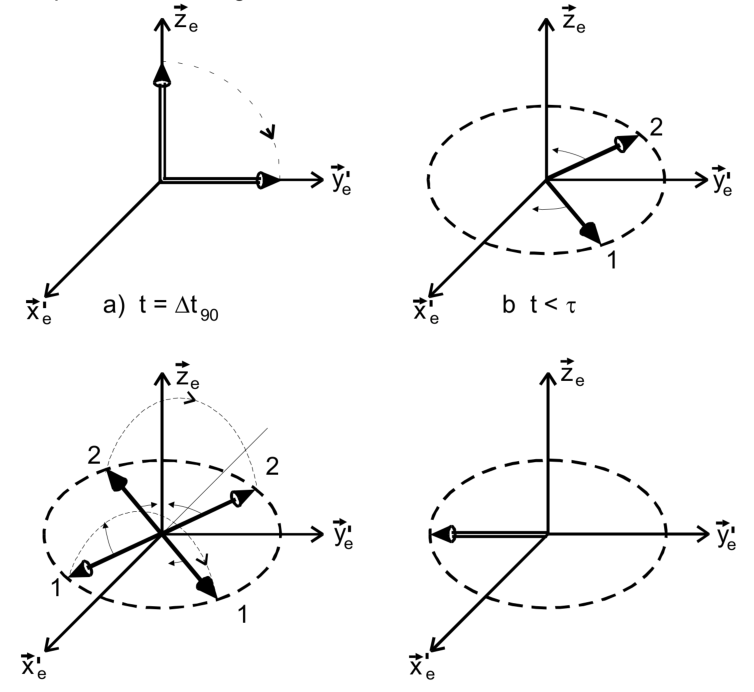
\includegraphics[width=.7\textwidth]{images/spin-echo-schema.pdf}
  \caption{Schematische Darstellung des Spin-Echo-Verfahrens im zeitlichen Verlauf \cite[9]{anleitung}.}
  \label{fig:Spin-Echo-Schema}
\end{figure}
Wie in den vorherigen Kapiteln beschrieben dephasieren die einzelnen Spins
aufgrund der Inhomogenität des statischen Magnetfeldes.
Im rotierenden Koordinatensystem rotieren die Spins mit größerer Larmorfrequenz als
das System im Uhrzeigersinn und die Spins mit kleinerer Larmorfrequenz
in die andere Richtung.
Dies ist durch zwei Zeiger in Abbildung \ref{fig:Spin-Echo-Schema} b) angedeutet.
Nach der Zeit $T_{\Delta B}$ ist praktisch keine transversale Magnetisierung messbar.
Aus diesem Grund wird nach einer einstellbaren Zeit $\tau$ ein
\SI{180}{\degree}-Puls auf die Probe gegeben, welcher die Spins wieder in die
$\vec{x}' \vec{y}'$-Ebene dreht, wie in Abbildung \ref{fig:Spin-Echo-Schema} c) dargestellt.
Aufgrund dieser Drehung laufen die Spins nun in der selben Geschwindigkeit aufeinander
zu, mit der sie zuvor dephasiert sind.
So lässt sich nach der Zeit $2 \tau$ eine transversale Magnetisierung in die
entgegengesetzte Richtung messen (siehe Abbildung \ref{fig:Spin-Echo-Schema} d)).
Dieses Echo wird Hahn-Echo genannt.
In Abbildung \ref{fig:Hahn-Echo} ist der gesamte erwartete Signalverlauf dargestellt.
\begin{figure}
  \centering
  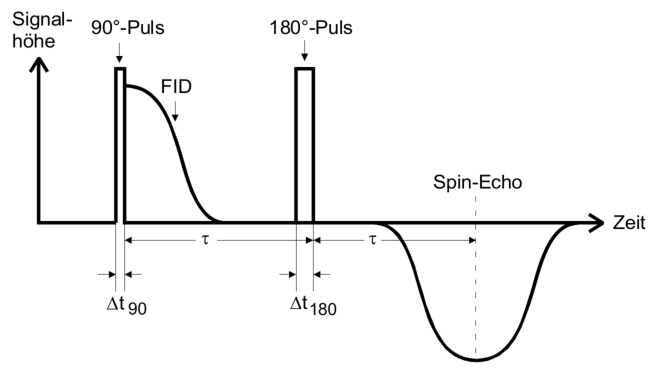
\includegraphics[width=.7\textwidth]{images/hahn-echo.pdf}
  \caption{Darstellung des Signalverlaufs des SEV \cite[9]{anleitung}.}
  \label{fig:Hahn-Echo}
\end{figure}
Da die transversale Magnetisierung wie in Abschnitt \ref{sec:TheoMagnetisierung}
beschrieben mit der Relaxationszeit $T_2$ zerfällt, hat das Spin-Echo nicht die
selbe Höhe wie der Eingangsimpuls bei $t = \SI{0}{\second}$.
Beschrieben wird dieser irreversible Zerfall durch
\begin{equation*}
  \frac{\symup{d} M_\text{y}}{\symup{d} t} = - \frac{M_\text{y}}{T_2}
\end{equation*}
mit den Anfangsbedingungen
\begin{equation*}
  M_\text{x} = M_\text{z} = 0 \quad \text{und} \quad M_\text{x} = M_0.
\end{equation*}
Diese Bedingung sind durch den Beginn des Zerfalls unmittelbar nach dem
\SI{90}{\degree}-Puls motiviert und führen auf den Zusammenhang
\begin{equation}
  M_\text{y}\!\left(t\right) = M_0 \exp\!\left(- \frac{t}{T_2}\right),
  \label{eqn:Spin-Echo-Statisch}
\end{equation}
nach welchem sich aus der Höhe des Spin-Echos in Abhängigkeit der
Zeit $\tau$ die Relaxationszeit $T_2$ bestimmen lässt.


\subsection{Die Carr-Purcell und Meilboom-Gill Methode}
\label{sec:CP-und-MG}

Die \emph{Carr-Purcell-Methode} (CPM) verwendet nach einem \SI{90}{\degree}-Impuls
eine Reihe von \SI{180}{\degree}-Impulsen im Abstand $2 \tau$, die jeweils
zu einer nachfolgenden Fokussierung der transversalen Magnetisierung führen.
Ein schematischer Signalverlauf ist in Abbildung \ref{fig:Carr-Purcell-Methode}
dargestellt.
\begin{figure}
  \centering
  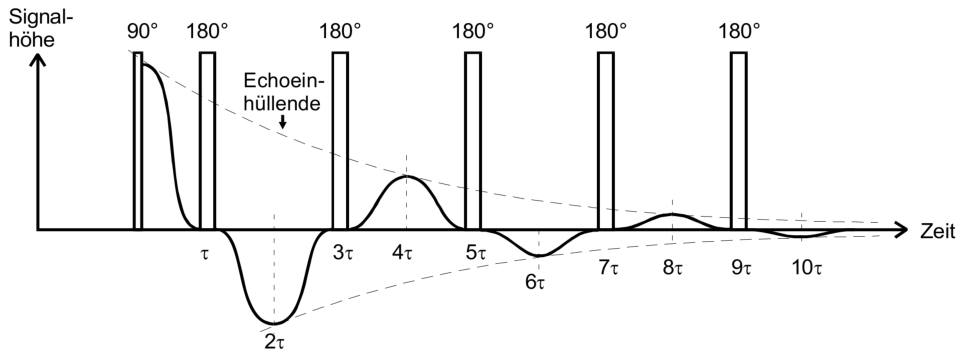
\includegraphics[width=.9\textwidth]{images/carr-purcell.pdf}
  \caption{Darstellung des Signalverlaufs bei der CPM \cite[11]{anleitung}.}
  \label{fig:Carr-Purcell-Methode}
\end{figure}
Diese Methode hat im Vergleich zum einfachen Spin-Echo
(Abschnitt \ref{sec:Spin-Echo-Verfahren}) den Vorteil, dass mehrere
Echos pro Messung vermessen werden können.
Wie im vorherigen Abschnitt beschrieben sinkt die Amplitude dieser Echos im
Laufe der Zeit aufgrund von Relaxationsprozessen.
Eine Schwierigkeit dieser Methode ist die exakte Einstellung der
\SI{180}{\degree}-Impulse.
Ist diese nicht gegeben, werden die einzelnen Spins nicht genau in die
$\vec{x}' \vec{y}'$-Ebene gedreht und die gemessene Magnetisierung
der $\vec{x}' \vec{y}'$-Ebene ist zu klein (und damit auch das erhaltene $T_2$).

Diese Problematik wird in der \emph{Meilboom-Gill-Methode} (MGM)
umgangen.
Wie bei der CPM folgen auf einen \SI{90}{\degree}-Impuls mehrere \SI{180}{\degree}-Impulse.
Hier wird jedoch die Schwingung in den \SI{180}{\degree}-Impulsen
um \SI{90}{\degree} gegen die \SI{90}{\degree}-Impulse phasenverschoben.
Folglich werden die einzelnen Spins nicht um die $\vec{x}'$-Achse,
sondern um die $\vec{y}'$-Achse gedreht, da $\vec{B}_1$ nun in die $\vec{y}'$-Achse zeigt.
Sind die \SI{180}{\degree}-Impulse nun nicht exakt eingestellt,
wird der Fehler $\delta$ durch den darauf folgenden Impuls wieder ausgeglichen.
In Abbildung \ref{fig:Meilboom-Gill-Methode} ist dieser Ausgleichprozess schematisch
dargestellt.
Abbildung \ref{fig:Meilboom-Gill-Methode} a) zeigt zwei exemplarische Spins,
die nach dem ersten \SI{180}{\degree}-Impuls
nicht exakt in die $\vec{x}' \vec{y}'$-Ebene gedreht wurden.
Somit ist gemessene transversale Magnetisierung
nach Abbildung \ref{fig:Meilboom-Gill-Methode} b) zu klein.
Werden die Spins in Abbildung \ref{fig:Meilboom-Gill-Methode} c) bei einem zweiten
\SI{180}{\degree}-Impuls wiederum gedreht, so gleicht sich der Fehler
wieder aus und die Refokussierung liegt wieder in der $\vec{x}' \vec{y}'$-Ebene.
Folglich besitzen anders als bei der CPM alle Echos das selbe Vorzeichen.
\begin{figure}
  \centering
  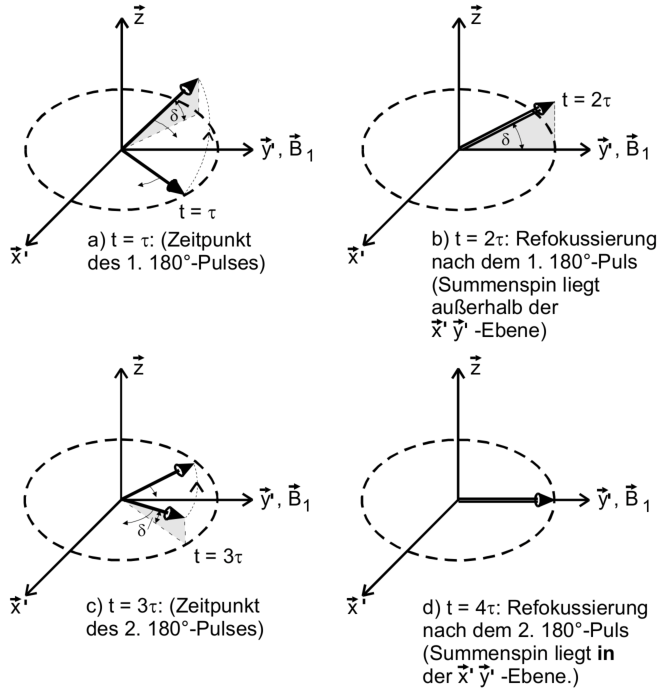
\includegraphics[width=.7\textwidth]{images/meilboom-gill.pdf}
  \caption{Schematische Darstellung der Refokussierung bei der MGM \cite[12]{anleitung}.}
  \label{fig:Meilboom-Gill-Methode}
\end{figure}


\subsection{Spinrelaxation einer flüssigen Probe}
\label{sec:DiffusionTheo}

In einer flüssigen Probe bewegen sich die Spins aufgrund der Brownschen
Molekularbewegung.
Dies hat zur Folge, dass das von den Spins wahrgenommene Magnetfeld
zeitlich veränderlich ist und Gleichung \eqref{eqn:Spin-Echo-Statisch} nicht mehr
anwendbar ist.
Eine adequate Beschreibung ist nur durch Ergänzung eines zusätzlichen Diffusionsterms
zu den Blochschen Gleichungen möglich.
Die Diffusionsstromdichte $\vec{j}$ (Anzahl Teilchen, die pro Zeiteinheit eine
Flächeneinheit durchqueren) ist gegeben durch
\begin{equation*}
  \vec{j} = - D\:\nabla\!\left(\frac{N}{V}\right)
\end{equation*}
mit der Diffusionskonstante $D$, der Teilchenzahl $N$ und dem Volumen $V$.
% Bei den hier betrachteten Protonen mit $S = \sfrac{1}{2}$ können die einzelnen
% Spins zwei Einstellungen haben (\textuparrow oder \textdownarrow).
Mit jedem Teilchen, dass das betrachtete Volumenelement verlässt und hinein kommt,
ändert sich die Magnetisierung.
Unter Verwendung des Gaußschen Integralsatzes lässt sich zeigen, dass
\begin{equation*}
  \frac{\partial M}{\partial t} = D\:\Delta M
\end{equation*}
gilt, wenn die Diffusionskonstante ortsunabhängig ist.
In Verbindung mit den Blochschen Gleichungen gilt dann
\begin{equation*}
  \frac{\partial M}{\partial t} =
  \underbrace{\gamma \left(\vec{M} \times \vec{B}\right)}_{\text{Präzession}}
  \underbrace{- \frac{M_\text{x} \vec{x} + M_\text{y} \vec{y}}{T_2}
  - \frac{\left(M_\text{z} - M_0\right) \vec{z}}{T_1}}_{\text{Relaxation}}
  \underbrace{+ \left(\vec{x} + \vec{y} + \vec{z}\right) D\:\Delta M}_{\text{Diffusion}}
\end{equation*}
für die Zeitentwicklung der Magnetisierung.
Für das gesamte Volumen der Probe wird
\begin{equation*}
  B_\text{z} = B_0 + G z
\end{equation*}
angesetzt, mit dem Feldgradienten des externen Magnetfelds $G$.
Dieser Feldgradient sei innerhalb der Probe konstant.
Unter diesen Annahmen lässt sich der Ausdruck
\begin{equation*}
  M_\text{y}\!\left(t\right) = M_0
  \exp\!\left(- \frac{t}{T_2}\right)
  \exp\!\left(- \frac{t}{T_\text{D}}\right)
\end{equation*}
mit
\begin{equation*}
  T_\text{D} = \frac{3}{D \gamma^2 G^2 \tau^2}
\end{equation*}
für die $y$-Komponente der Magnetisierung gewinnen.
Hierbei ist $\tau$ die in Abschnitt \ref{sec:CP-und-MG} eingeführte Zeit zwischen
dem \SI{90}{\degree}- und dem \SI{180}{\degree}-Impuls.
Aufgrund der Diffusion ergibt sich also ein zweiter exponentieller Faktor, der
zum Zerfall der Magnetisierung beiträgt.
Die CPM und die MGM aus Abschnitt \ref{sec:CP-und-MG} können weiterhin
angewandt werden, wenn $T_\text{D}$ groß gegen $T_2$ ist.
Des Weiteren gilt bei Betrachtung der Signalhöhe des ersten Spin-Echos
\begin{equation}
  M_\text{y}\!\left(t\right) = M_0
  \exp\!\left(-\frac{t}{T_2}\right)
  \exp\!\left(-\frac{1}{12} D \gamma^2 G^2 t^3\right)
  \label{eqn:DiffusionsBestimmung}
\end{equation}
mit $t = 2\tau$,
woraus sich bei Variation von $t$ die Diffusionskonstante ermitteln lässt.


\subsection{Bestimmung der Relaxationszeit \texorpdfstring{$T_1$}{T1}}
\label{sec:T1Theo}

Die longitudinale Relaxationszeit $T_1$ kann auf eine ähnliche Weise wie die
transversale Relaxationszeit bestimmt werden.
Ein \SI{180}{\degree}-Impuls dreht alle Spins aus der $\vec{z}$-Richtung in
die negative $\vec{z}$-Richtung. Im zeitlichen Verlauf relaxieren die Spins zurück
in die $\vec{z}$-Richtung (Gleichgewichtslage).
Nach der Zeit $\tau$ dreht ein \SI{90}{\degree}-Impuls die verbliebene Magnetisierung
der $-\vec{z}$-Richtung in die $\vec{x}'\vec{y}'$-Ebene.
Dort präzedieren die einzelnen Spin und induzieren damit eine Spannung, die
proportional zur Magnetisierung ist.
Aus den Blochschen Gleichung ergibt sich mit den Anfangsbedingungen
\begin{equation*}
  M_\text{x}\!\left(0\right) = M_\text{y}\!\left(0\right) = 0
  \quad \text{und} \quad M_\text{z}\!\left(0\right) = M_0
\end{equation*}
für die Magnetisierung in $\vec{z}$-Richtung
\begin{equation}
  M_\text{z}\!\left(\tau\right) =
  M_0 \left(1 - 2 \exp\!\left[-\frac{\tau}{T_1}\right]\right)
  \label{eqn:T1-Vermessung}
\end{equation}
durch Integration.
Wird $M_\text{z}$ für verschiedene Zeiten $\tau$ gemessen, lässt sich aus diesem
Zusammenhang $T_1$ bestimmen.
